\documentclass{school-22.101-notes}
\date{December 7, 2011}

\begin{document}
\maketitle

\topic{Charged Particle Interaction}
\begin{align}
    P_e &= \int \dt \frac{Ze^2}{x^2 + b^2} \frac{b}{\sqrt{x^2 + b^2}} \\
    &= \int_{-\infty}^{\infty} \frac{2e^2}{x^2+b^2} \frac{b}{\sqrt{x^2 + b^2}} \frac{\dx}{v} \\
    &\approx \frac{2e^2 b}{v} \int \frac{\dx}{(x^2 + b^2)^{3/2}} = \frac{2Ze^2}{vb} \\
    \frac{P_e^2}{2m} &= \frac{2 (Ze^2)^2}{m_e b^2 v^2} \\
    \mbox{Stopping Power} &= - \frac{\dE}{\dx} = \int_{b_{min}}^{b_{max}} n2(2 \pi b) \derivative b \frac{2}{m_e} \left( \frac{2e^2}{vb} \right)^2 \\
    &= \frac{4 \pi (Ze^2)^2nZ }{m_e v^2 } \ln \left( \frac{b_{max}}{b_{min}} \right) \\
    &= \frac{4 \pi Z^2 e^4 n Z}{m_e v^2} \ln \left( \frac{2 m_e v^2}{\bar{I}} \right) 
\end{align}
Relativistic Stopping Power, `Bethe Formula' (correction to the above equation to include high energy):
\eqn{- \frac{\dE}{\dx} = \frac{4 \pi Z^2 e^4 nZ}{m_e v^2} \left[ \ln \left( \frac{2 m_e c^2 \beta^2}{I (1-\beta^2) } \right) - \beta^2 \right]   }
collision with nucleus: $-\frac{\dE}{\dx}$ increases by factor of Z; decreases by factor of $\frac{m_e}{M[Z]}$. 

Range:
\begin{align}
    R &= \int_0^R \dx = \int_{E_0}^0 \frac{\dx}{\dE} \dE = \int_0^{E_0} \left( - \frac{\dE}{\dx} \right)^{-1} \dE 
\end{align}
In the $\frac{1}{v^2}$ range, $R \sim \int_0^{E_0} E \dE = E_0^2$. 
In the log/real range, $R\ sim \int_0^{E_0} \dE  = E_0$. 
A good rule of thumb to remember about comparing two particles' range:
\eqn{ \frac{R_1 (v)}{R_2 (v)} = \frac{Z_2^2 M_1}{Z_1^2 M_2} }

Range of validity:
\begin{itemize}
    \item $E \gg 500 \bar{I}$. 
    \item $\frac{Z e^2}{\hbar v} = \left( \frac{e^2}{\hbar c} \right) \frac{Z}{v/c} = \frac{Z}{137 (v/c) } \ll 1 $
\end{itemize}

\subtopic{Cerenkov Radiation}
Typically, $v_{light} = \frac{c}{n}.$ For instance, speed of light in water is 0.75c. When $v> \frac{c}{n}$, we see the blue glow in ractors that are water cooled. 



%\begin{figure}
%   \centering
%   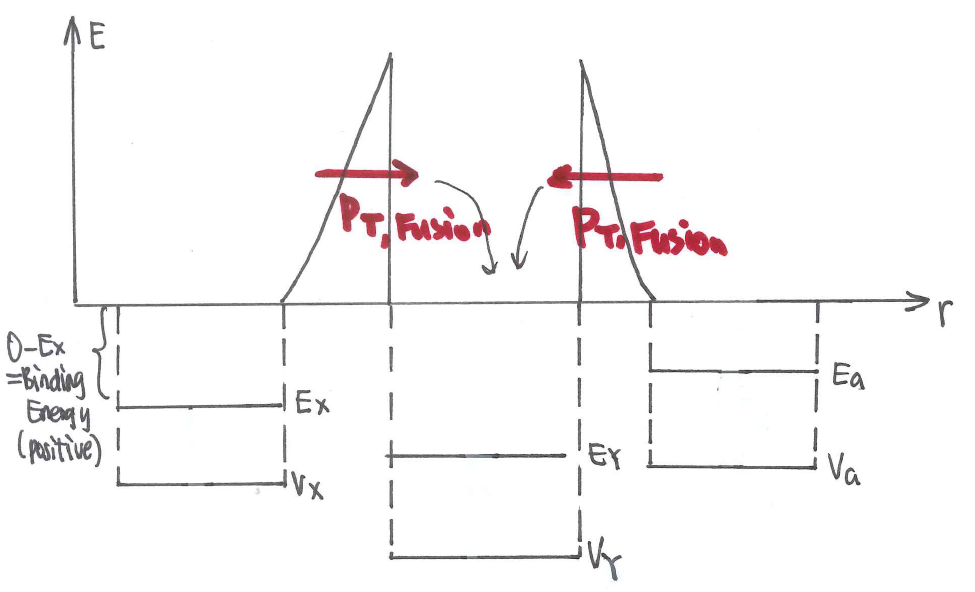
\includegraphics[width=4in]{images/ni/fusion-mechanism.png}
%   \caption{Mechanism for Fusion\label{fusion-mechanism}}
%\end{figure}



\end{document}
